\documentclass[preprint]{sigplanconf}

% The following \documentclass options may be useful:
% preprint      Remove this option only once the paper is in final form.

\usepackage{amsmath}
\usepackage{graphicx}
\usepackage{hyperref}
\usepackage{url}

\newcommand{\ALGOL}{A\textsc{LGOL}}
\newcommand{\MATLAB}{\textsc{MATLAB}}
\newcommand{\Mathematica}{\textit{Mathematica}}
\newcommand{\code}[1]{\texttt{#1}}

\begin{document}

\special{papersize=8.5in,11in}
\setlength{\pdfpageheight}{\paperheight}
\setlength{\pdfpagewidth}{\paperwidth}

\conferenceinfo{ARRAY '14}{June 15, 2014, Edinburgh, UK}
\copyrightyear{2014} 
%\copyrightdata{978-1-nnnn-nnnn-n/yy/mm} 
%\doi{nnnnnnn.nnnnnnn}

% Uncomment one of the following two, if you are not going for the 
% traditional copyright transfer agreement.

%\exclusivelicense                % ACM gets exclusive license to publish, 
                                  % you retain copyright

\permissiontopublish             % ACM gets nonexclusive license to publish
                                  % (paid open-access papers, 
                                  % short abstracts)

\titlebanner{Julia Arrays for Modern Technical Computing}    % These are ignored unless
\preprintfooter{Julia Arrays for Modern Technical Computing} % 'preprint' option specified.

% \title{Array implementations in Julia}
% \subtitle{Implementing arrays in a way that is amenable to compiler analysis}

\title{Julia Arrays for Modern Technical Computing}
\subtitle{ Managing Efficiency/Flexibility and Abstraction/Specialization Tradeoffs through Multiple Dispatch}
\authorinfo{Jeff Bezanson \and Jiahao Chen \and Keno Fischer \and Alan Edelman}
           {MIT Computer Science and Artificial Intelligence Laboratory}
           {\{ bezanson, jiahao, kfischer, edelman \}@csail.mit.edu}

%TODO Get Dahua to sign on as coauthor
%\authorinfo{Dahua Lin}
%           {Toyota Technological Institute at Chicago}
%           {dhlin@ttic.edu}

\maketitle

\begin{abstract}
This is the text of the abstract.
\end{abstract}

%\category{CR-number}{subcategory}{third-level}

\keywords
Julia, multiple dispatch

\section{Introduction}

\begin{quotation}
``Unfortunately, it is very difficult for a designer to select in advance all
the abstractions which the users of his language might need. If a language is
to be used at all, it is likely to be used to solve problems which its
designer did not envision, and for which abstractions embedded in the language
are not sufficient.'' - Ref. \cite{Liskov:1974pb}
\end{quotation}

One-dimensional arrays are a simple and essential data structure found in most
programming languages. The multi-dimensional arrays required in scientific
computing, however, are a different beast entirely. Allowing any number of
dimensions entails a significant increase in complexity. Why? The essential
reason is that core properties of the data structure no longer fit in a
constant amount of space. The space needed to store the sizes of the
dimensions (the array shape) is proportional to the number of dimensions. This
does not seem so bad, but becomes a large problem due to three additional
facts:

\begin{enumerate}

\item{\bf Efficiency:} Code that operates on the dimension sizes needs to be
highly efficient. Typically the overhead of a loop is unacceptable, and such
code needs to be fully unrolled.

\item{\bf Dynamic Nature:} In some code the number of dimensions is a
\emph{dynamic} property --- it is only known at run time.

%TODO is this really a point about static vs dynamic arrays?

\item {\bf Dimension Specialization:} Programs may wish to treat arrays with
different numbers of dimensions very differently. A vector---an intrinsically
one-dimensional object---is conceptually very different from an $N\times1$
matrix, which is intrinsically two-dimensional. For example, it may be important
in certain applications to distinguish between vector norms and certain types
of matrix norms. Also, certain computations like the singular value decomposition
make sense only for matrices, not vectors. These differences in object semantics
and behavior make the number of dimensions a crucial part of program semantics and
thus cannot be merely a compiler implementation detail. Even though it is possible
to construct an isomorphism between column vectors and $N\times1$ matrices,
semantic differences preclude a genuine ``is-a'' relationship, and hence violates
the Liskov substitution principle \cite{Liskov:1987da}. We can think of this
situation as the linear algebraic counterpart to the canonical circle-ellipse
problem \cite{Halbert:1987ut}.

%TODO Something here about transposition?

\end{enumerate}

These facts pull in different directions:

\begin{enumerate}

\item Efficiency begs for static analysis.

\item Dynamic properties call for run-time flexibility. 

\item Dimension specialization suggests that dimensionality should be part of the type system, but partly determined at run time (for example, via virtual method dispatch).

\end{enumerate}

Current approaches choose a compromise. In some systems, the number of
dimensions has a strict limit (e.g. 3 or 4), so that separate classes for each
case may be written out in full. Other systems choose flexibility, and just
accept that most or all operations will be dynamically dispatched. Other
systems might provide flexibility only at compile time, for example a template
library where the number of dimensions must be statically known.

%% TODO: examples of systems limited to n==3

Whatever decision is made, rules must be defined for how various operators act
on dimensions. For now we will focus on indexing, since selecting parts of
arrays has particularly rich behavior with respect to dimensionality. For
example, if a single row or column of a matrix is selected, does the result
have one or two dimensions? Array implementations prefer to invoke general
rules to answer such questions. Such a rule might say ``dimensions indexed
with scalars are dropped'', or ``trailing dimensions of size one are
dropped'', or ``the rank of the result is the sum of the ranks of the
indexes'' (as in APL).

\subsection{Array implementations in other languages}

\subsubsection{FORTRAN}

Arguably, arrays were the earliest data structure to be conceived of, and
implemented on, computers, dating back to Konrad Zuse's Plankalk\"ul
\cite{Zuse:1948ua, Rojas:2000pk}. However, the first implementation of arrays
in a high-level language was described in the reference implementation of
FORTRAN I on the IBM 704 \cite{Backus:1957fa}, where static arrays of up to
three dimensions were allowed. The programmers' manual
\cite[pp.~10--11]{Backus:1956pr} describes that:

\begin{enumerate}
\item The elements of the array are stored sequentially in memory.
\item The elements are in column-major order.
\item The elements are stored from bottom right to top left.
\end{enumerate}

From this we can see that the first array language specification to be
actually implemented specified that arrays were to be stored in a linear
contiguous block in memory, that it was strided backward in memory and in
column major style, and it had associated metadata about its shape which was
partly user-controllable: the maximal rank was 3 (hard coded) \footnote{The
maximal rank of an array was increased to 7 in Fortran 77, and later to 15 in
Fortran 2008.}, but the size in each dimension could be user-specified. The
design decisions of the semantics of arrays were hard coded into the FORTRAN I
compiler, and have guided the design of compilers ever since.

%CITE Compilers textbook

Static arrays are conceptually simple: a contiguous block of memory storing
elements of identical sizes allows element indices to be computed at runtime
efficiently and random access can happen in essentially O(1) time. At the same
time, reducing the constant prefactor for index-to-offset computations lead to
nontrivial compiler design challenges for efficient implementation, such as
common subexpression elimination for computing strides, and loop fusion for
certain types of array traversal \cite{Busam:1969oe}.

%TODO Fortran started with only arrays; objects were added later: Arrays were
%the only compound type supported by Fortran. In Fortran however, arrays were
%a fundamental part of the language from the very beginning, whereas objects
%were not introduced until the advent of Object-Oriented Fortran and Fortran
%2003.

\subsubsection{ALGOL 60}

The arrays in Fortran were static arrays, where the size of the array is known
and fixed at compile time and cannot be changed at runtime. \footnote{Dynamic
arrays were introduced in the Fortran 90 standard with the \code{ALLOCATABLE}
keyword.} In contrast, the contemporaneous \ALGOL{} 60 programming language
supported dynamic multidimensional arrays: not only were the arrays of
arbitrary rank, but the size of the array could also change at runtime. This
posed a challenge for compiler writers of the time. They introduced what was
called the \textit{dope vector} \cite{Sattley:1960as, Sattley:1961as}, which
contained the size and lower bound of each dimension, and the closely related
\textit{storage mapping function} \cite[pp.~80--87]{Randell:1964a6} for the
special case of 0-based indices and is essentially equivalent to
\code{size(A::Array)} in Julia; both contain information needed to convert
from the multidimensional array index to a linear memory offset.

\subsubsection{C}

C, like Fortran before Fortran 90, traditionally supports static arrays only,
which are allocated on the stack. In practice, however, C can support dynamic
arrays also: memory on the heap can be dynamically allocated and assigned a
pointer \cite{Kernigham:1978cp}. Dynamic arrays created in this way, however,
must implement array semantics manually, requiring the programmer to implement
indexing and striding by hand using pointer arithmetic, and manually
propagating information such as the extent of the trailing dimension, is can
be lost at function call boundaries. To this extent, C takes a minimalist
approach to arrays, where all components of array semantics must be
implemented manually.

There are two different ways you can implement dynamic multidimensional arrays
in C. You can implement arrays of arrays, which thanks to the equivalence of
pointer arithmetic and array indexing in C \textit{in one dimension}
\cite[pp.~93--96]{Kernigham:1978cp}, can support the \code{A[i][j]} indexing
semantics of static arrays. However, arrays of arrays are strictly speaking
not true arrays because the memory is not guaranteed to be contiguous in
memory. Alternative you can \code{malloc} a contiguous block of memory with a
single pointer, but the pointer arithmetic \code{*(\&A[0]+i)} supports only a
single index corresponding to the raw memory offset, and you will have to do
the indexing arithmetic manually for multidimensional arrays.

% In some sense, C does not have a disjunction between arrays and other
% objects. In C, objects and arrays can only be accessed semantically with
% pointers. To the extent that C has a minimalist approach to both objects and
% arrays, they are not disjoint.

\subsubsection{C++}

% You can try to use the object system in C++ to implement arrays, but it's a
% disaster.

C++ does not introduce a fundamentally new way to handle arrays. One might
argue that dynamic and static arrays are implemented by the \code{std::vector}
and \code{std::array} classes of the C++ Standard Library. However, the
semantics are hard coded for one dimension only. Furthermore, directly
indexing a vector \code{a[i]} is not required to incur a bounds check (such
behavior is undefined by the standard), but only with the more cumbersome
syntax \code{a.at(i)}, which then throws an \code{std::out\_of\_range}
exception if \code{i} is out of bounds. In principle, a container resembling
multidimensional arrays can be created by chaining these classes together,
forming syntactically awkward constructions like
\code{std::vector<std::vector<...>>}. However, this strictly speaking is not
an array data structure if one consider a contiguous memory store to be one of
the defining features of arrays, as there is no guarantee that C++ will
allocate memory in this fashion. Additionally, the distinction made between
\code{vector}s and \code{array}s in principle could lead to very strange
constructs that are static in some dimensions but dynamic in others, e.g. in
the chain \code{std::vector<std::array<...>>}. Furthermore such nested constructs
do not interoperate well with other parts of the C++ standard library such as
iterators or even \code{max\_element}, thus limiting their usefulness
\cite{Bavestrelli:2000ct}.

In practice, the high cost of iterative containers means that such constructs
are not widely used; instead, programs use C-style arrays or resort to
external libraries like \code{Blitz++} \cite{Veldhuizen:1998ab} or
\code{Boost.MultiArray} \cite{Garcia:2005ma}, which use complicated
template metaprogramming techniques to achieve performance.

Boost MultiArrays are completely defined by four properties: the memory
address of the origin element, shape, index bases (first index in each
dimension), and strides \cite{Garcia:2005ma}. In particular, the stride
specification allows for arrays to be stored in row-major or column-major
order (or their multidimensional generalizations) as desired.

%% TODO: insert example of limited power of C++ array libraries

\subsubsection{Mathematica}

In \Mathematica, the central data type is an expression
\cite{mathematica:expr}, whose parts can be referenced by the
\code{[[]]}, or \code{Part}, symbol \cite{mathematica:part}: \code{A[[0]]}
returns the head of the expression, and \code{A[[i]]} returns the $i^{th}$
argument. At the discretion of the internal compiler, \Mathematica{} arrays
may be represented internally as expression trees, with each level of the tree
represented as a continguous array of pointers first to the head and then to
each part, or as ``packed arrays of machine-sized integers or real numbers'',
a description which resembles the traditional array data structure
\cite{mathematica:int}. To the user, however, arrays are simply nested lists
\cite{mathematica:nl}, and the \code{[[]]} symbol naturally lends itself to
the role of array indexing.

The implementation of \Mathematica{} arrays as nested lists has two non--obvious
consequences. First, it is possible to ``index'' an array with more
indices than its rank; the extra indices would simply traverse into the
expression contained within the matrix element. For example, \code{Array[f,
{3, 4}][[3, 2]]} returns \code{f[3,2]}, whilst \code{Array[f, {3, 4}][[3, 2,
1]]} returns \code{3}. Thus the semantics of the \code{Part} symbol is more
general than pure array indexing and allows for violations of the array data
abstraction, which may come as a surprise to users. Second, \Mathematica{}
interprets nested lists of depth $n$ as rank-$n$ multidimensionary arrays
(which are termed ``tensors'' in \Mathematica), but at the same time
implicitly assumes the isomorphism between, say, rank-4 arrays and matrices of
matrices, which \Mathematica{} takes advantage of when displaying results in
\code{MatrixForm}. For example, the code
\begin{verbatim}
Zero[n_] := Table[0, ##] & @@ Table[{2}, {n}]
\end{verbatim}
generates the zero array of rank $n$ and size (2,2,\dots,2), which when 
displayed in \code{MatrixForm} will render as nested matrices and vectors, as 
demonstrated in Figure~\ref{fig:mathematica}.

\begin{figure}
  \centering
  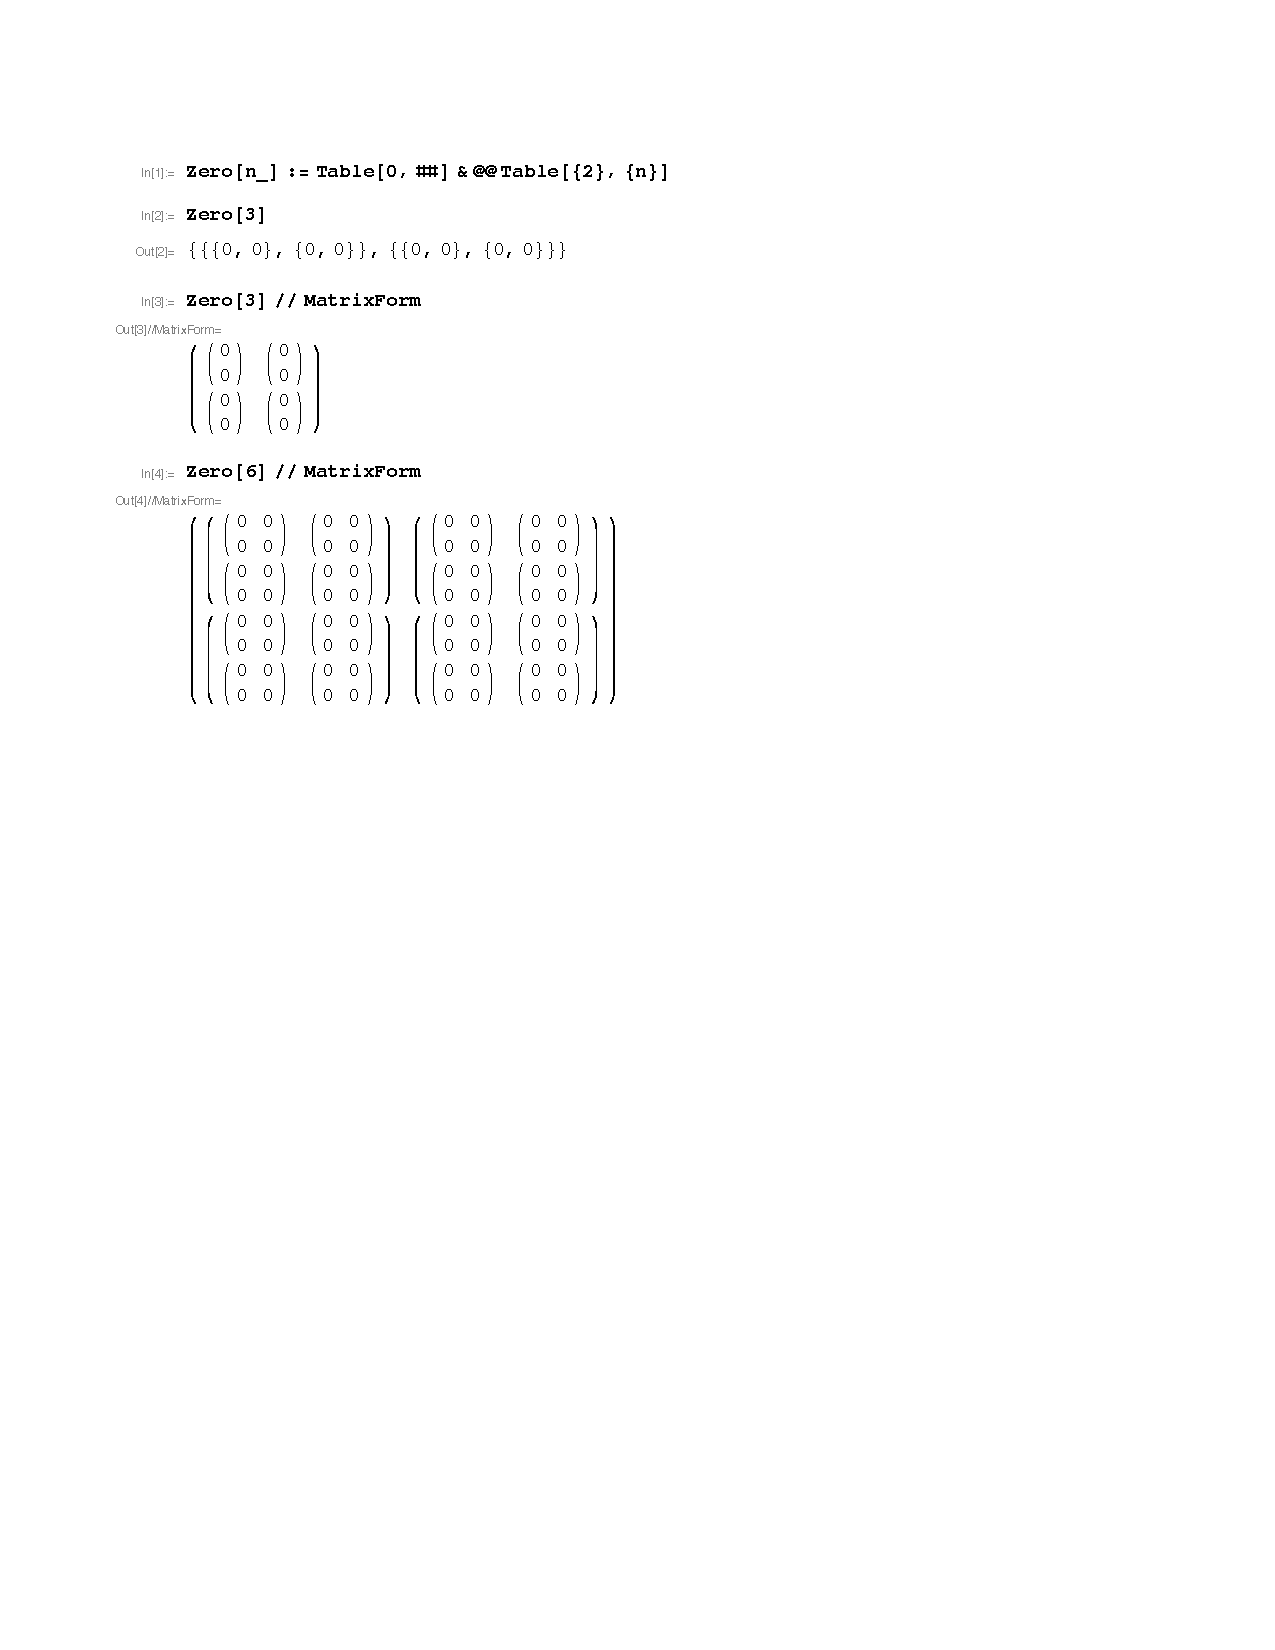
\includegraphics[width=\columnwidth]{fig-mathematica/fig.pdf}
  \caption{\label{fig:mathematica} Creating and displaying the zero array of
rank $n$ and size (2,2,\dots,2). ($n=3$ and $n=6$ shown.) \Mathematica's
\code{MatrixForm} function nests two dimensional structures.}
\end{figure}

\subsubsection{MATLAB}

Arrays are the most fundamental data type in \MATLAB{}, and all \MATLAB{}
arrays must have at least two dimensions. Consequently, row vectors, column
vectors and scalars are treated as isomorphic to matrices with dimensions
$1\times N$, $N\times1$ and $1\times1$ respectively. This reflects \MATLAB's
original design principle as a ``\textbf{matrix} laboratory".

Not having pure scalars can be mathematically troublesome. For example, the
product $A_{m\times n} \times B_{1\times 1} \times C_{n\times p}$ is invalid
under the ordinary rules of matrix multiplication for $n\ne1$; however,
\MATLAB{} would allow the evaluation of this product by interpreting $B$ as a
scalar which commutes with $A$ and $C$, allowing this product to be evaluated
as the product of the scalar $B_{11}$ and the matrix product $A_{m\times n}
\times C_{n\times p}$.

%TODO Find examples where this kind of interpretation breaks commutativity or
%associativity. Matrices of matrices or matrices of quaternions?

Also, all arrays are treated as if they have an infinite number of trailing
singleton dimensions. This reflects a later design decision in \MATLAB{} to
support multilinear algebra \cite{matlabman:ma},  albeit in a manner that does
not quite mesh with the world of ordinary linear algebra. This unfortunately
clashes with the \textit{linear indexing} rule in \MATLAB{} that indexing a
multidimensional array with a single index automatically triggers a reshape.
For example, for $A_{3\times4}$, there is an ambiguity as to whether
\texttt{A(5)} means \texttt{B=A(:);B(5)} or \texttt{A(5,1,1,\dots)}, and this
ambiguity can only be resolved by performing a runtime bounds check as a
consequence of an arbitrary design decision.

\MATLAB{} also allows indexing with matrices, but they are treated as if they
were flattened for indexing purposes, i.e.
\begin{verbatim}
A(M1, M2, dots) = A(M1(:), M2(:)), dots
\end{verbatim}

There is also something very funky with \MATLAB's cell arrays. You have to
index into them using \texttt{A\{...\}} instead of the usual \texttt{A(...)}.

%TODO Find an example for which this causes problems?

Problems for static compilers for dynamics languages? Matlab in particular?

%\subsubsection{R}

%\subsubsection{APL}

%\subsubsection{ZPL}

%\subsubsection{Python/NumPy}

Problems with dynamic language implementations? Python?

\subsubsection{Summary}

Arrays suffer from dearth of abstraction - lots of manual implementation, hand
coded into the compiler, implementation is imposed on users. Oftentimes the
object system is disjoint from the arrays, e.g. R types, because these
subsystems were tacked onto the language at different points in time. In
NumPy, mechanisms of objects are not well used. Detailed manual mechanisms in
C code. Custom dispatch, generated code, pretty crazy. NumPy arrays are Python
objects but the mechanism of the object system don't play a huge role in
defining behavior. Objects are lookup tables of behaviors, primarily centered
around indexing behavior. Single indexing lookup of symbols which are just
integers. Not very powerful - people think it is because it is dynamic
dispatch. We can generalize it to be tremendously more powerful.

Implementation details: row vs column major, indexing rules, etc., constrain
how users have to deal with stuff.

\section{Julia Arrays}

Julia uses the object system to implement arrays. Arrays are implemented as
the \code{Array} data type, which is parametric on the \code{Type} of element
it contains, and also its rank (which defaults to 1). Internally,
\code{Array}s are implemented as a pair of (shape, linear data storage) =
metadata of bounded size O(1) + raw data O(N). This basic structure is
sufficient to define the semantics of multidimensional arrays, yet is flexible
to incorporate a wide range of nontrivial design decisions.

One of the core features of Julia is multiple dispatch. Consequently, it is
possible for \code{Array}s to have implementations that afford both generality
and efficiency. The most general \code{Array\{Any\}} is an associative array
implemented as an array of pointers to heap-allocated values. However,
\code{Array}s of native machine types like double precision floating point
numbers (\code{Float64}s) or integers of native machine size (\code{Int}s) can
be implemented to be C/Fortran-compatible. Interestingly,
\code{Array\{Nothing\}} can be implemented with zero storage space at runtime,
since it consists of elements of an immutable type with zero fields, which is
possible because only a single instance of any such type can exist, and hence
need not actually be stored. This allows for some clever tricks like
implementing \code{Set\{T\}} using a \code{Dict\{T,Nothing\}} to avoid paying
any cost for the value array in the \code{Dict}.

%TODO This superficially resembles the N-dimensional class template of
%Bavestrelli:2000ct. But \code{Array<T,N>} is defined recursively using
%C++ templates and 
%\code{operator[]} to produce \code{Array<T,N-1>}, etc., down to the base case
%of \code{Array<T,1>} which has to be explicitly specified. Furthermore, C++'s
% semantics for \code{operator[]} means that indexing must recurse from
%leftmost to rightmost index.

%Jeff: A big difference is that templates require manually specifying
%what to do at compile time vs. run time. They are effectively a
%separate language. A single, all-run-time model is much easier to use.
%Templates are not available at run time, so you are restricted in what
%kinds of code you can write. For example in julia you can do `A[I...]`
%where `I` is a heterogeneous array, and all the same definitions are
%still applicable, but you might take a bit of performance drop.

%Jeff: In the past, language abstraction mechanisms
%were not powerful enough to define N-d arrays. The behaviors had to be
%built in to the compiler (or inside a very elaborate C library like
%numpy). In julia, method signatures plus a general-purpose (not
%array-specific) type inference algorithm can do it. The combination
%turns out to be very important: if you only have multiple dispatch,
%you just have a nifty-but-slow way to write these things. If you just
%have type inference, then you are quite limited in what you can
%realistically infer --- for example an explicit loop over the
%arguments to getindex is too dynamic, and you can't really infer what
%it does.

%TODO Comment on how Mathematica claims to have multiple implementations of
%Arrays too, but this is not within the purvey of the end user's control.

%TODO where does this fit? Stefan: Part of this story is our support for
%immutable types since you need two things to allow this: a parametric array
%type and immutable types to put into it. One other feature that's necessary
%is that concrete types are final. You can accomplish this in other languages
%by declaring these types to be final, but we don't have to.

Here we consider the indexing rules. How to compute shapes of subarrays. How
to deal with singleton dimensions is but a very special case even though
superficially the rules mention them explicitly.

Here is a good place to use Julia code to codify all the various indexing
rules that various languages have

In Julia, such indexing rules are defined in exactly one place and can be
changed later if so desired.

\subsection{The need for flexibility in array indexing rules}

Our goal here is a bit unusual: we are not concerned with which rules might
work best, but merely with how they can be specified, so that domain experts
can experiment.

In fact different domains want different things. E.g. in images, each
dimension might be quite different, e.g. time vs. space vs. color, so you
don't want to drop or rearrange dimensions very often.

In practice we may all have to reach a consensus on what rules to use, but it
should not be enforced upon uses by pure technical implementation convenience.
The point is that in Julia, these are not enforced a priori. Sometimes the
distinctions between the various indexing rules are semantically meaningful
and that's when this flexibility becomes particularly valuable. For example
Tim Holy's image 4-arrays. Quantum mechanics when you average out multiple
indistinguishable particles. $n$-point correlations functions where which $k$
indices you average out defines any number of lower-point $n-k$ point
correlation functions.

\subsection{Ground rules}
Here are our ground rules:

\begin{enumerate}
\item You can't manually implement the behavior inside the compiler
\item The compiler must be able to reasonably understand the program
\item The code must be reasonably easy to write
\end{enumerate}

How are such rules implemented? For a language with built-in multidimensional
arrays, the compiler will analyze indexing expressions and determine an answer
using hard-coded logic.

% TODO: grab example from one of these compilers

However, this approach is not satisfying: we would rather implement the
behavior in libraries, so that different kinds of arrays may be defined, or so
that rules of similar complexity may be defined for other kinds of objects.
But these kinds of rules are unusually difficult to implement in libraries. If
a library writes out its indexing logic using imperative code, the host
language compiler is not likely to be able to analyze it. Using compile-time
abstracton (templates) would provide better performance, but such libraries
tend to be difficult to write (and read), and the full complement of indexing
behavior expected by technical users strains the capabilities of such systems.

% TODO: insert actual example of numpy

Our dispatch mechanism permits a novel solution. If a multiple dispatch system
supports variadic functions and argument ``splicing'' (the ability to pass a
structure of $n$ values as $n$ separate arguments to a function), then
indexing behavior can be defined as method signatures.

This solution is still a compromise among the factors outlined above, but it
is a new compromise that provides a net-better solution.

% TODO more

\section{\texttt{index\_shape}}

Below we define a function \texttt{index\_shape} that computes the shape of a
result array given a series of index arguments. We show three versions, each
implementing a different rule that users in different domains might want:

% TODO: point out array = (shape, data), so those are the two parts we need to
% handle. In julia the ``data'' part is not a first class object; it is not
% directly exposed to the user, but this is more of an implementation detail.

\begin{verbatim}
# drop dimensions indexed with scalars
index_shape() = ()
index_shape(i::Real, I...) = index_shape(I...)
index_shape(i, I...) = tuple(length(i), index_shape(I...)...)
\end{verbatim}

\begin{verbatim}
# drop trailing dimensions indexed with scalars
index_shape(i::Real...) = ()
index_shape(i, I...) = tuple(length(i), index_shape(I...)...)
\end{verbatim}

\begin{verbatim}
# rank summing (APL)
index_shape() = ()
index_shape(i, I...) = tuple(size(i)..., index_shape(I...)...)
\end{verbatim}

Inferring the length of the result of \texttt{index\_shape} is sufficient to
infer the rank of the result array.

These definitions are concise, easy to write, and possible for a compiler to
understand fully using straightforward techniques.

% TODO: point out how this combines the ``object part'' and the ``array part''
% into a coherent whole.

%TODO put in some cleaned-up version of Jeff's derivation of the first case.

The result type is determined using only dataflow type inference, plus a rule
for splicing an immediate container (the type of \texttt{f((a,b)...)} is the
type of \texttt{f(a,b)}). Argument list destructuring takes place inside the
type intersection operator used to combine argument types with method
signatures.

This approach does not depend on any heuristics. Each call to
\texttt{index\_shape} simply requires one recursive invocation of type
inference. This process reaches the base case \texttt{()} for these
definitions, since each recursive call handles a shorter argument list (for
less-well-behaved definitions, we might end up invoking a widening operator
instead).


\begin{verbatim}

diverge() = randbool() ? () : tuple(1, diverge()...)

\end{verbatim}

\section{Array views (Dahua's stuff)}

Also interesting are array views. In certain cases of subarray slicing, it is
possible to keep the data in place and return just a view (pointer) to the
data instead of creating a new copy in memory. In this case the same
infrastructure that applies to full arrays automatically works for subarrays.
Views are just another thing that implement the array protocol: (length, size,
getindex). Is there a point here about code reuse? Maybe but Jeff thinks it's
not crucial.


\section{Extensions of the idea}

If we redefine Array to be (shape, stride pattern and linear data store), this
would be sufficient to extend to row major vs column major. We would have a
language that is majorization-agnostic, which defies the traditional
classification.

Data locality is another interesting issue. This can be part of the definition
of Arrays. Data locality is an open problem. Maybe we need multiple linear
data stores. Maybe we need complicated locality maps to be part of the
associated metadata. But the point is that with a flexible definition in the
Base library, not hard-coded into the compiler, these are design decisions
that can be revisted and modified if necessary.

Locality and majorization order are two facets of the more general issue -
where are the data located? With the right abstractions you can implement and
experiment with them, change them without too much difficulty. We may not have
all the answers but you can experiment with the possibilities in the same
spelling.

Another interesting possibility is the treatment of symmetric and
antisymmetric tensors, since the ability to define custom striding rules would
allow for representations of such quantities that eliminate the redundant
storage of symmetry-equivalent components. (This becomes very important in
higher dimensions $d$ since multiplicity of redundant storage grows as
O($d!$).

%TODO missing theme: There's also a big question about whether arrays are
%static or dynamic. (immutable vs mutable types)

%Stefan: The bottom line for whether something should be mutable or not is
%psychological: is the thing a value or a container? Integers are naturally
%immutable. If you modify an integer, you don't have the same integer with a
%different value, you have a different integer. If you have two distinct
%integers with the same value, they're not different, they're just different
%copies of the same integer. Arrays, on the other hand, are naturally mutable.
%If you have an array and you change the value in its first slot, you still
%have the same array, just with different contents. Similarly, you can have
%two different arrays that happen to contain the same values, but that doesn't
%make them the same array.

%\appendix
%\section{Appendix Title}
%
%This is the text of the appendix, if you need one.

\acks

The authors gratefully acknowledge the enthusiastic participation of the Julia
developer community for many stimulating discussions on the topic of array
implementations in the Julia language.

%TODO thank Intel, Wade, and perhaps NSF Solar here

% We recommend abbrvnat bibliography style.

\bibliography{refs}{}
\bibliographystyle{abbrvnat}

% The bibliography should be embedded for final submission.

%\begin{thebibliography}{}
%\softraggedright

%\bibitem[Smith et~al.(2009)Smith, Jones]{smith02}
%P. Q. Smith, and X. Y. Jones. ...reference text...

%\end{thebibliography}

\end{document}
